\documentclass[../SimBALink.tex]{subfiles}

\graphicspath{ {./Model/Powertrain/Battery_pack/Documentation/Figures/}{../Model/Powertrain/Battery_pack/Documentation/Figures/} }
\begin{document}
\subsection{Block diagram}
soon

\subsection{Inputs and outputs}
	\subsubsubsection{Inputs}
\begin{tabular}{ r | c | l | l }
		Signal						&	Symbol		&	MATLAB variable	&	Unit						\\\hline
		DC current					&	$I_{dc}$		&	\texttt{Idc}		&	A		\\
	\end{tabular}
	
	\subsubsubsection{Outputs}
\begin{tabular}{ r | c | l | l }
		Signal						&	Symbol				&	MATLAB variable	&	Unit						\\\hline
		State of charge				&	SOC					&	\texttt{SOC}		&	\%		\\
		Terminal voltage				&	$V_{dc}$				&	\texttt{V}			&	V		\\
	\end{tabular}
	
\subsection{Background, rationale, modeling strategy}
	\subsubsubsection{Electrical model}
		Each battery cell is modeled as an equivalent circuit:
		
		\begin{figure}[h!]
				\centering
				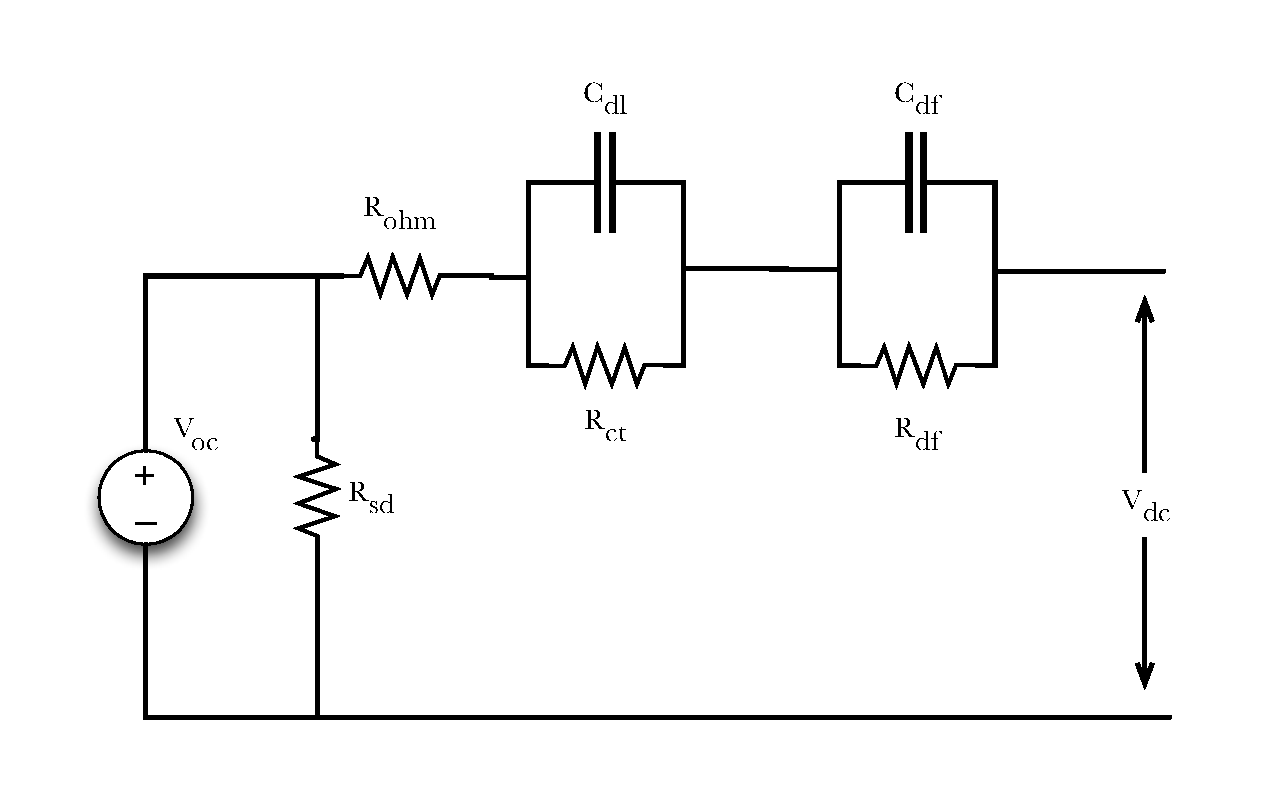
\includegraphics[width=4in]{Battery_pack_equivalent_circuit}
				\caption{Battery cell equivalent circuit}
				\label{fig:battery_pack_equivalent_circuit}
		\end{figure}
		\FloatBarrier
		
		where:
		\begin{center}
		\begin{tabular}{l l}
			$V_{oc}$		&	is the battery open-circuit voltage in volts	\\
			$R_{0}$		&	is the battery zero-order resistance (AC resistance) in ohms \\
			$R_{1}$		& 	is the battery first-order resistance in ohms \\\
			$C_{1}$		&	is the battery first-order capacitance in farads \\
		\end{tabular}
		\end{center}
		
		The battery open-circuit voltage, $V_{oc}$, is a function of the remaining cell capacity Q, and is represented by a lookup table.
		
		For a series circuit composed of $n$ identical battery cells, the terminal voltage of the series circuit is $n \times V_{oc}$.
		
	\subsubsubsection{Thermal model}
		The battery pack thermal model is not implemented. It is assumed that the battery open-circuit voltage has no temperature dependence.
		

\subsection{Parameters}
	\begin{tabular}{ r | l | l | l }
		Parameter				&	Symbol				&	MATLAB variable	&	Unit						\\	\hline	
		Initial stored charge			&	$Q_0$				&	\texttt{Q\_0}		&	coulomb					\\
		Number of series cells		&	n					&	\texttt{n}			&							\\
		Zero-order series resistance	&	$R_0$				&	\texttt{R0}			&	ohm						\\
		First-order capacitance		&	$C_1$				&	\texttt{C1}			&	farad					\\
		First-order resistance		&	$R_1$				&	\texttt{R1}			&	ohm						\\
		Open-circuit voltage			&	$V_\text{oc}(\text{SOC})$&	\texttt{Voc}		&	volt						\\
		Open-circuit voltage lookup: state-of-charge breakpoints	&		&	\texttt{Voc.SOC}	&							\\
		Open-circuit voltage lookup: voltage data	&			&	\texttt{Voc.V}		& 	volt
	\end{tabular}

\subsection{Assumptions}
	This battery pack model assumes that:
	
	\begin{itemize}
		\item		None of the equivalent-circuit parameters are affected by temperature.		
		\item		The charging and discharging open-circuit voltage profiles are identical.	
	\end{itemize}	

\end{document}